\section{Teórico}

  \definicion{Topic:} Time-dependent density-functional perturbation theory.

  \definicion{Speaker:} Iurii TIMROV (EPFL, Switzerland).

Ver la foto de suite of codes para ponerla en el día 1.

\subsection{Espectroscopia computacional: desde el estado basal hacia estados excitados}

  Todo lo visto hasta ahora permite describir el estado fundamental. Ahora queremos ver qué ocurre cuando excitamos los elecctrones para que pasen desde la banda de valencai hacia la banda de conducción, por ejemplo.

  Para que los cálculos sean comparables con los experimentos, debemos incluir el dominio temporal en los mismos.

\subsection{Ecuación de Schrödinger dependiente del tiempo}

  Se sigue considerando la aproximación BO como en el caso estático. La ecuación de Schrödinger dependiente del tiempo establece la evolución de un sistema no relativista many-electrons interactuantes: no sólo se agrega la derivada temporal, sino que además se incorpora la variación temporal al término del potencial externo del Hamiltoniano del sistema.

  En vez de considerar las funciones de onda de $3N+1$ variables (3N posiciones más el tiempo), nuevamente consideramos la densdiad electrónica, la cual es una función de $4$ variables:
    $$n (\vec{r}, t) = N \int \norm{}^2$$

  Mientras que DFT es un mapeo uno-a-uno entre la densidad de carga y el potencial externo estático, mediante minimización de la energía total, [...]

\subsection{Teoremas de Runge-Gross}

  El primer teorema establece que [...]

  Permite establecer una relación unívoca (monomorfismo) entre el potencial externo y la densidad electrónica. Todos los observables son funcionales de esta densidad de carga dependiente del tiempo. La diferencia es que necesitamos una CI.

  En TDDFT no podemos formular un principio variacional.

  [...]

  El segundo teorema establece que [...]

  Es posible resolver el problema dependiente del tiempo buscando el punto estacionario de la acción. Este no necesariamente tiene que ser mínimo, sino que simplemente necesita ser un extremo. El valor de la acción en sí no ofrece información extra ya que se anula [...]

\subsection{Funcional de acción mecano-cuántico}

  Cinético, Hartree y XC. El último es el potencial externo (se le agrega la dependencia del tiempo).

  El término de Hartre tiene una expresión como la estática, pero se le agrega el tiempo.

  Para aproximar el funcional de acción, Gross y Kohn introdujeron un sistema auxiliar de partículas no interactuantes que satisfacen las ecuaciones KS dependientes del tiempo: ahora el potencial efectivo depende también del tiempo.

  [...]

  \Obs{Es lo que hicieron KS a partir de HK en el caso independiente del tiempo.}

  \Obs{Pensar en el formalismo de Lagrange.}

\subsection{Aproximación adiabática}

  En el caso dependiente del tiempo, el potencial XC depende del tiempo y de la densidad $n (\vec{r}, t)$ en todo momento pasado, dando lugar a una expresión mucho más compleja. La elección más usada es conocida como ALDA (Adiabatic LDA), la cual es obtenida a partir de evaluar el potecial LDA con la densidad $n (\vec{r}, t)$.

  [...]

  Limitaciones: [...]

\subsection{TDDFPT: Linear-response TDDFT}

  En TDDFT tenemos dos regímenes extremos: el de respuesta lineal y el de respuesta no lineal, los cuales dependen de si la perturbación es débil o fuerte, respectivamente.

  En el caso del régimen lineal, las ecuaciones TDDFT se resuelven tanto en el dominio temporal o en [...]

  [...]

  Asumimos entonces que el potencial externo depende del tiempo, pero es débil.

  [...]

  Expandimos la densidad en serie de Taylor a primer orden.

  [...]  chi es la susceptibilidad del material. Es no local (dos r). Depende de la diferencia temporal.

  Se trata de TDDFT en conjunto con la teoría perturbacional y por eso se abrevia como TDDFPT.

  Existen al menos 4 métodos de linearizar y calcular la susceptibilidad para TDDFPT:
    \begin{enumerate}
      \item \textbf{Método de Dyson:} la susceptibilidad es la variación de la densidad de carga respecto al potencial externo. Haciendo la regla de la cadena, se introduce el potencial KS con unas integrales. Éste a su vez es descripto como tres derivadas: de Hartree, de XC y de unas deltas de Dirac. Reescribe la variación del potencial de Hartree y del potencial XC (XC kernel). Se llega a que la susceptibilidad depende de sí mismma. Juntando todos los resultados se llega a una ecuación tipo Dyson, donde el término no integral se conoce como la polarizabilidad independiente de partículas. Esta última función tiene picos cuando el denominador se anula: la energía del fotón entrante $\hbar\omega$ se iguala con la diferencia entre niveles $\epsilon_i - \epsilon_j$ (la singularidad se levanta con una cantidad infinitesimal Lorentziana).
      [...]

      Al pasar al espacio recíproco mediante FT pasamos de una ecuación integral a una ecuación matricial, con $q$ y $\omega$ fijos. A veces la ecuación se resuelve en la RPA (Random Phase Approxmation) donde se descarta la contribución XC.
      [...]

      Con DFT obtenemos la polarizabilidad independiente de partículas y luego con el método de Dyson obtenemos la susceptibilidad.

      Problemas:
        - Sumar sobre estados vacíos para $\chi^0$. Estos son infinitos, hay que saber dónde cortar para la convergencia. Caro.
        - Multiplicación e inversión de matrices muy grandes. Caro.
        - Ambas matrices $\chi$ y $\chi^0$ deben ser resueltas para cada frecuencia de interés. Caro.

      No está disponible en QE por todos estos problemas. Hay otras técnicas más avanzadas implementadas.
      \item \textbf{Método de Sternheimer:} escribimos el potencial externo como el término fundamental más la contribución dependiente del tiempo. Lo mismo para el potencial XC. Esto lleva a que el Hamiltoniano KS se pueda escribiir como una contribución fundamental más una contribución dependiente del tiempo. Esto lleva a que los estados KS son la suma del estado KS fundamental y [...], todo multiplicado por una fase temporal. A partir de esto reescribimos la ecuación KS en las ecuaciones de Sternheimer: una resonante y una antiresonante.
        [...]

      Para resolverlas hacemos FT para ir del dominio temporal al de frecuencias.
        [...]

      \Obs{Si las frecuencias fueran nulas y los potenciales no dependieran de las frecuencias, las ecuaciones caen en el caso de DFPT para el cálculo de fonones.}

      potencial Coulómbico + XC. n prima es la densidad respuesta. El factor de 2 es por la degeneración para materiales no polarizados.

      Vemos de vuelta que se muerde la cola: la densidad respuesta depende de las funciones de onda que son autoestados de las ecuaciones. Debemos recurrir a SCF.

      Lo bueno es que no necesitamos considerar estados vacíos ya que los proyectores sobre estados vacíos se pueden reescribir en términos de los proyectores sobre los estados ocupados. Sin embargo, seguimos necesitando resolver todo para cada frecuencia.
      \item \textbf{Método de Liouville-Lanczos:} parte de la ecuación cuántica de Liouville que describe la evolución temporal del operador densidad de carga, la cual depende únicamente de las bandas de valencia. Usando teoría de respuesta lineal, se expande a primer orden la ecaución de Liouville.
        [...]

      Luego definimos el superoperador de Liouville y pasamos al dominio de frecuencias la ecuación linealizada.
        [...]

      La solución formal a esta ecuación es mediante inversión matricial según
        [...]

      Finalmente, la susceptibilidad del operador $A$ en función dela frecuencia será la traza del producto entre el observable y la densidad.

      En la práctica esto se resuelve recurriendo al método recursivo de Lanczos. Se define un standard batch representation: la semisuma y la semiresta de las fuciones de onda. [...] Con esto reescribimos todo en términos de un producto matricial.

      [...] deinfe D y K

      Luego se definen dos vectores de Lanczos bidimensionales y la cadena de recursión de Lanczos, junto a los coeficientes de Lanczos. Al resolverla se general una matriz tridiagonal: es una matriz nula salvo en las diagonales $\pm 1$ respecto a la diagonal principal. Finalmente, una vez que tenemos esta matriz construida podemos calcular la susceptibilidad buscada (sea hace PP y no es costoso).

      En resumen:
        - No necesitamos considerar estados vacíos (misma razón que antes).
        - La matriz tridiagonal se computa sólo una vez y es independiente de la frecuencia.
        - El PP no es caro. Además la extrapolación de los coeficientes de Lanczos permite acelerar los cálculos.
      \item \textbf{Método de Casida-Davidson:} las ecuaciones de Casida parten de las ecuaciones de Sternheimer y anulan uno de sus miembros. Luego resuelve el problema de autovalores mediante un algoritmo de diagonalización tipo Davidson. Los autovalores corresponde a los polos de la susceptibilidad.
    \end{enumerate}

    Mientras que el método de Sternheimer es útil para sólidos, el método de Casida es útil para sistemas moleculares, ya que no es práctico en sólidos debido a la alta densidad de estados que éstos presentan. El método de Liouville es útil tanto para sólidos como para moléculas.

\subsection{Esepctroscopias}

  \begin{itemize}
    \item \textbf{Absorción óptica:} consideremos una perturbación externa asociada a un campo eléctrico homogéneo. Esta perturbación induce linealmente un dipolo. La conexión entre el dipolo generado y el campo aplicado es mediante el tensor de polarizabilidad dinámica (matriz 3x3).
    \item \textbf{Electron energy loss en sólidos:} ahora la perturbación no es un fotón, sino un electrón (una onda plana). Se mide el scaterring de los electrones.
    \item \textbf{Scattering inelástico de neutrones en sólidos:} ahora la perturbación es un neutrón, por lo que necesitamos considerar campos magnéticos. [...]
  \end{itemize}

\subsection{Aspectos generales}

  \begin{itemize}
    \item TDDFPT permite el modelado de una gran variedad de espectroscopias a un costo computacional relativamente bajo en comparación con teorías many-body.
    \item
    \item
  \end{itemize}

  [...]

\section{Q\&A}

\section{Hands-on}

  \definicion{Topic:} TDDFPT.

  \definicion{Speaker:}	Iurii TIMROV (EPFL, Switzerland), Oscar BASEGGIO (SISSA, Italy).

\subsection{Example 1}

  Habla muy lento y estuve perdido arreglando el ingreso al cluster. REVISAR.

  Switch on the electronic interaction (Hartree and Exchange-Correlation)

  El pico en torno a 8 eV es la siguiente excitación (de mayor energía).

  Tarda bastante más en hacer la turbo davidson ahora: de segundos a 6 minutos pasó.

  El de interacciones es un pico mini en torn a las 6.5 eV.

  \begin{figure}[H]
      \centering
      \subfigure[]{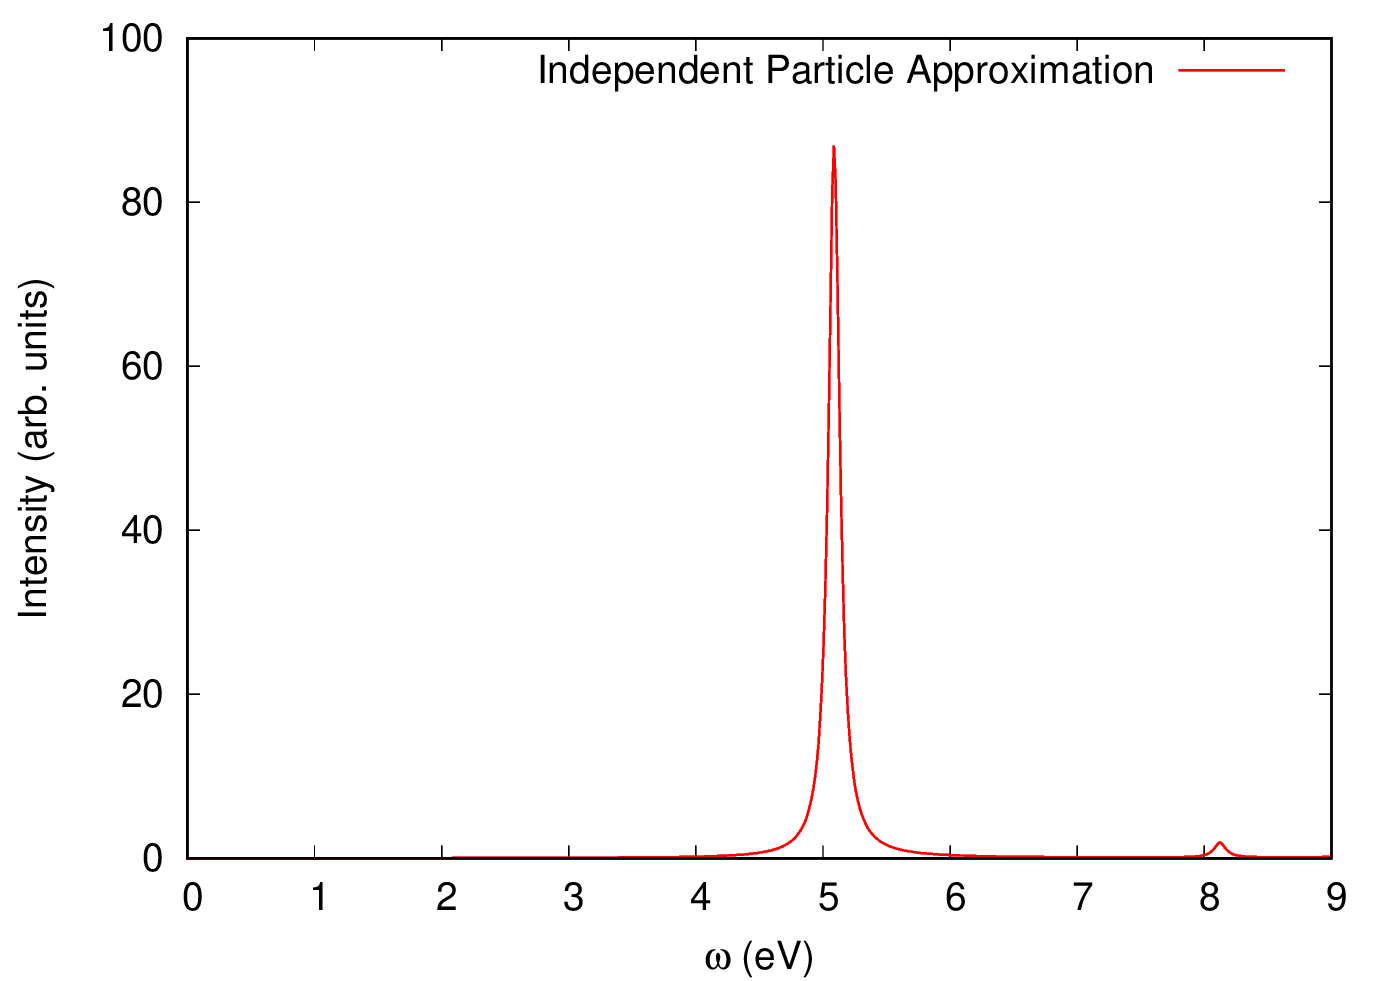
\includegraphics[scale = 0.3]{figs/D6/C6H6_pre.png}}
      \subfigure[]{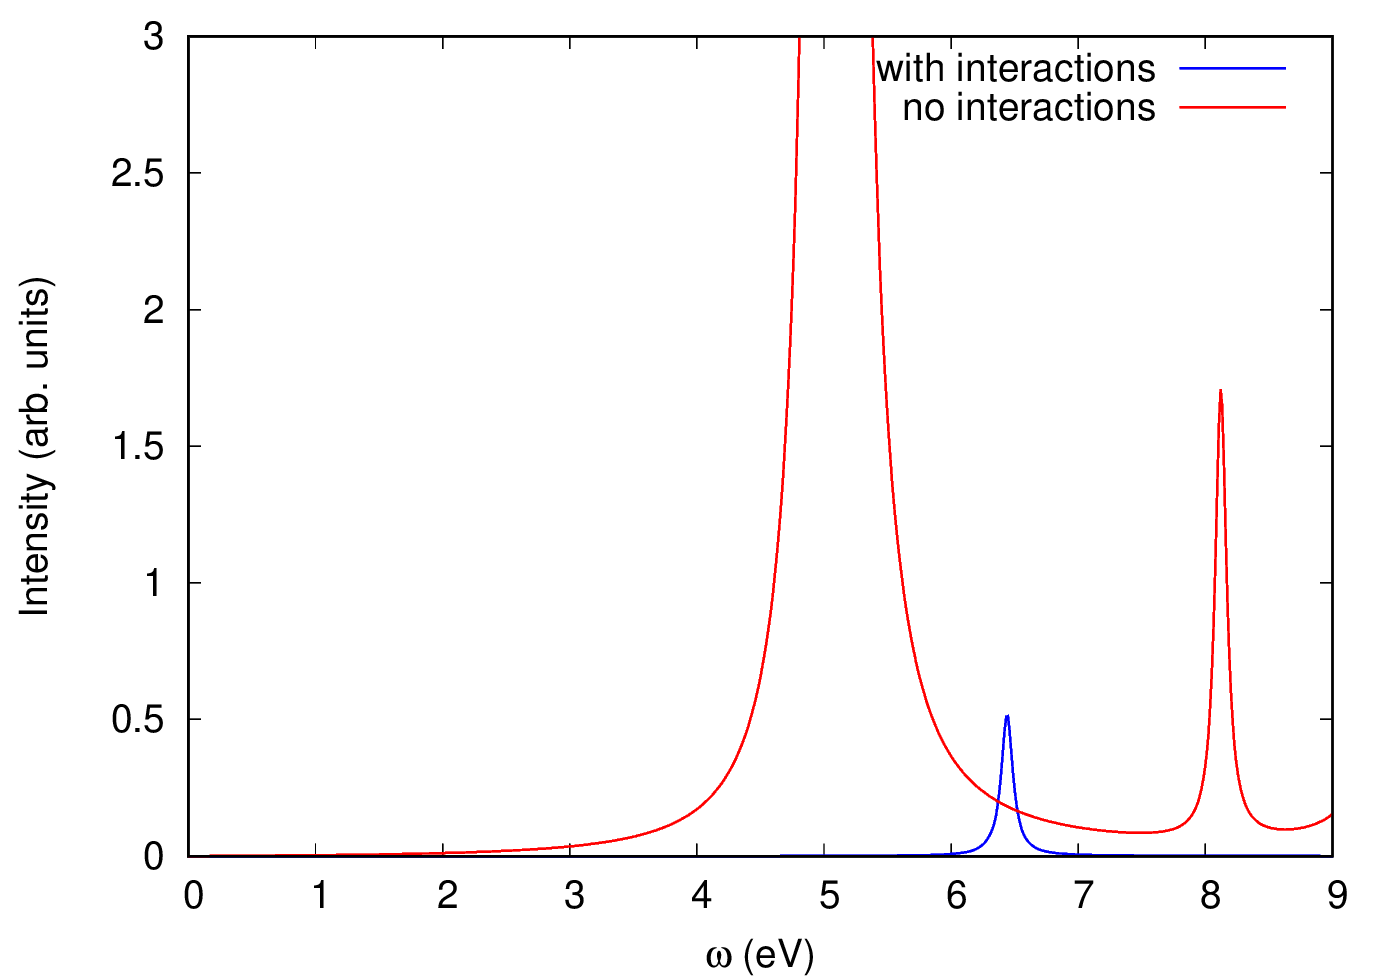
\includegraphics[scale = 0.3]{figs/D6/C6H6_post.png}}
      \caption{antes y después}
  \end{figure}

\subsection{Example 2}

  Esoectro: se pueden poner menos de la cantida total de iteraciones hechas, pero no más.

  A mayor cantidad de iteraciones va cambiando la ubicación de los picos. También cambian sus intensidades. Esto habla de que el espectro no está convergedio correctamente: hay que hacer más iteraciones o hacer un truco.

  Para el truco ver qué le pasa el beta de Lancszos: una extrapolación que aumenta el número de coeficientes sin calcularlos.

\subsection{Example 3}

  Los dos primeros estudiaban una molécula. Ahora vamos a estudiar un sólido.

  El calculator le dice si usar Lancszos o Sternheimer.

  q1, q2 y q3: componentes de la transferencia de momento.

  [me fui un buen tiempo]

  Siempre conviene hacer extrapolación porque ahorra una banda de tiempo.

  La definición del plasmon dice que el pico (de la imaginaria) ocurre en torno a la raíz de la parte real con pendiente positiva. Cuando la pendiente es negativa hay picos en le epsilon imaginaria.

\subsection{Example 4}

  Ejemplo más complejo de toda la escuela. Dos métodos bien distintos dan lugar a exactamente el mismo espectro.

  No tenemos las iteraciones (específicas de Lanczos), pero mantenemos las coordendasd del vector q. Hay otras palabras claves.

  Tarda unas 2 horas ya que no está del todo optimizado el código todavía.

  Dan igual espectro, pero el Lanczos le pasa el trapo en velocidad al Sternheimer. Aparece discreto porque hace un cálculo por frecuencia. Para tener un espectro más denso: más caro que eia.

  Obviamente que la convergencia de la k mesh hacerla con Lanczos. AL principio no es smooth pero a medida que avanza se suaviza.

  Dispersión plasmónica: el espectro va cambiando según el valor de la transferencia de momento. La dispersión plasmónica es la parábola que se forma al tomar las intensidades de los picos. 
